\documentclass{article}
\usepackage{color}
\usepackage{graphicx}
\usepackage{setspace}

\usepackage{geometry}
\usepackage{amsmath}
\usepackage{enumitem,amssymb}
\usepackage{pifont}
\definecolor{darkgreen}{rgb}{0.0, 0.5, 0.0}
\geometry{left = 1.25in, right=1.25in} % New Stuff Learned!
\newcommand{\cmark}{\ding{51}}
\newcommand{\xmark}{\ding{55}}
\newcommand{\done}{\rlap{$\square$}{\raisebox{2pt}{\large\hspace{1pt}\cmark}}
\hspace{-2.5pt}}
\newcommand{\wontfix}{\rlap{$\square$}{\large\hspace{1pt}\xmark}}
\newlist{todolist}{itemize}{2}
\setlist[todolist]{label=$\square$}
\doublespacing
\begin{document}
\begin{titlepage}
	

\title{\textbf{CHE374 Week 1}}
\author{\textit{Sanzhe Feng}}
\date{\textit{\today}}
\maketitle
\end{titlepage}
\setlength{\parindent}{0pt}

\section*{Interest Rate}
- Understand the concept of \textbf{interest} and \textbf{interest rate}

- Understand why interest is charged and factors that impact interest rate value

\subsection*{Basic Ideas}

- Borrowing money has a cost for the borrower

- Lending money should create value for the lender

- $F = P + NPi (I)$ where P is \emph{amount of money today} (also called \textit{Principle}), F is \emph{fucture amount}, N is time and i is \emph{\textbf{interest rate}}.
Note that we expect a higher payoff (F) in the future as the interest rate increases. Conversely, for a given F, as the interest rate increases,
the present value (P) decreases.

- Typically, a loan to government or bank will have lower interest rate but ``risk-free''. On the other hand, 
personal loans are much more risky but with significantly higher interest rates.

\subsection*{Factors than Affect Interest Rates}

- Inflation: Prices generally tend to increase over time; Higher expected inflation generally leads to an increase in interest rates.\\

- Credit (default) risk: Risk associated with the borrower being able to pay interest and principal. Higher risk of default leads to higher interest rates.\\

- Liquidity risk: Risk associated with being able to access the invested funds during the duration of the investment. The greater the liquidty risk, the less liquid the investment, the higher the interest rate.
Liquidity is the ability of a firm, company, or even an individual to pay its debts without suffering catastrophic losses.\\

- Maturity risk: Risk associated with the time horizon of the investment. The longer the maturity, the longer the investment payoff, which also increases credit (and potentially liquidity) risk leading to higher interest rates.\\

\section*{Simple and Compound Interest}
- Know why interest is charged

- \textbf{Calculate simple and compund interest}

\subsection*{Simple vs Comound Interest}

- Simple interest rate applies ONLY to the original principal

- Compound interest applies to the principal AND to all interest already accrued. $F_N = P(1+i)^N$ where $N$ is time.\\
\begin{center}
    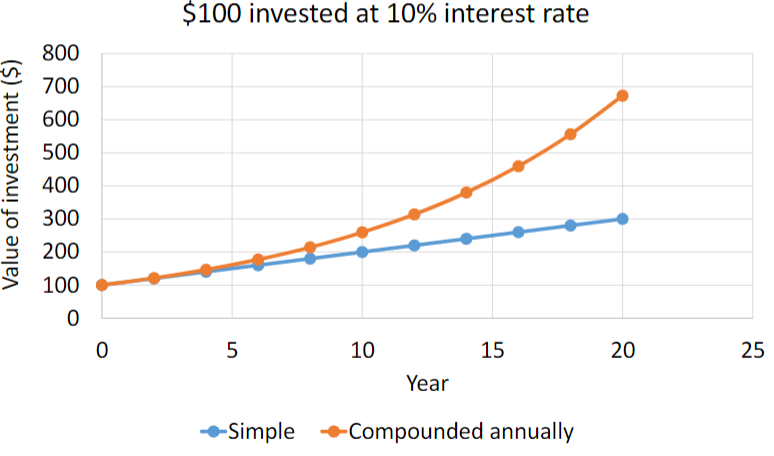
\includegraphics[width=0.8\linewidth]{W1V2.png}
\end{center}

\section*{Subperiod compounding and effective interest rate}

- Calculate subperiod interest rate and effective interest rate given the nominal interest rate and compounding period./

\subsection*{Compound multiple times per year}

$r$: Nominal interest rate (usually for 1 year), we compound m times per year:
\[F = P(1+\frac{r}{m})^m\]
The subperiod interest rate $i_s$ is a fraction of the nominal interest rate $\frac{r}{m}$.
Note that: the more frequently you compound (greater m), the more interest will earn. 


\subsection*{Effective interest rate}

Case 1: r = 6\%, compounded monthly; 

Case 2: r = 6.3\%, compounded once a year.

How do we know which to choose?
\textbf{Effective interest rate $i_e$}: the equivalent interest rate of an account is compounded just once over the stated time period (usually 1 year).  
\[ i_e = (1+\frac{r}{m})^m - 1\]

\subsection*{Continuous Compounding}
- As we shorten our compounding period, $i_e$ increase.

- But there is a limit for infinitesimally small period, known as \textbf{continous compounding}:
\[i_e = \lim_{m\to\infty}(1 +\frac{r}{m})^m - 1 = e^r -1\]

\end{document}
